\documentclass{article}
\usepackage[T1]{fontenc}
\usepackage{helvet}
\renewcommand{\familydefault}{\sfdefault}
\usepackage{amsmath,amssymb}
\usepackage{sansmath}
\usepackage{tikz}
\usetikzlibrary{arrows.meta,fit,calc,positioning}
\pagestyle{empty}
\definecolor{acc}{HTML}{1F4E79}
\newsavebox{\figbox}
\newcommand{\DD}{\mathord{\text{\fontencoding{OT1}\fontfamily{cmss}\selectfont\char1}}}
\begin{document}
\sansmath\fontsize{7}{8.4}\selectfont
\sbox{\figbox}{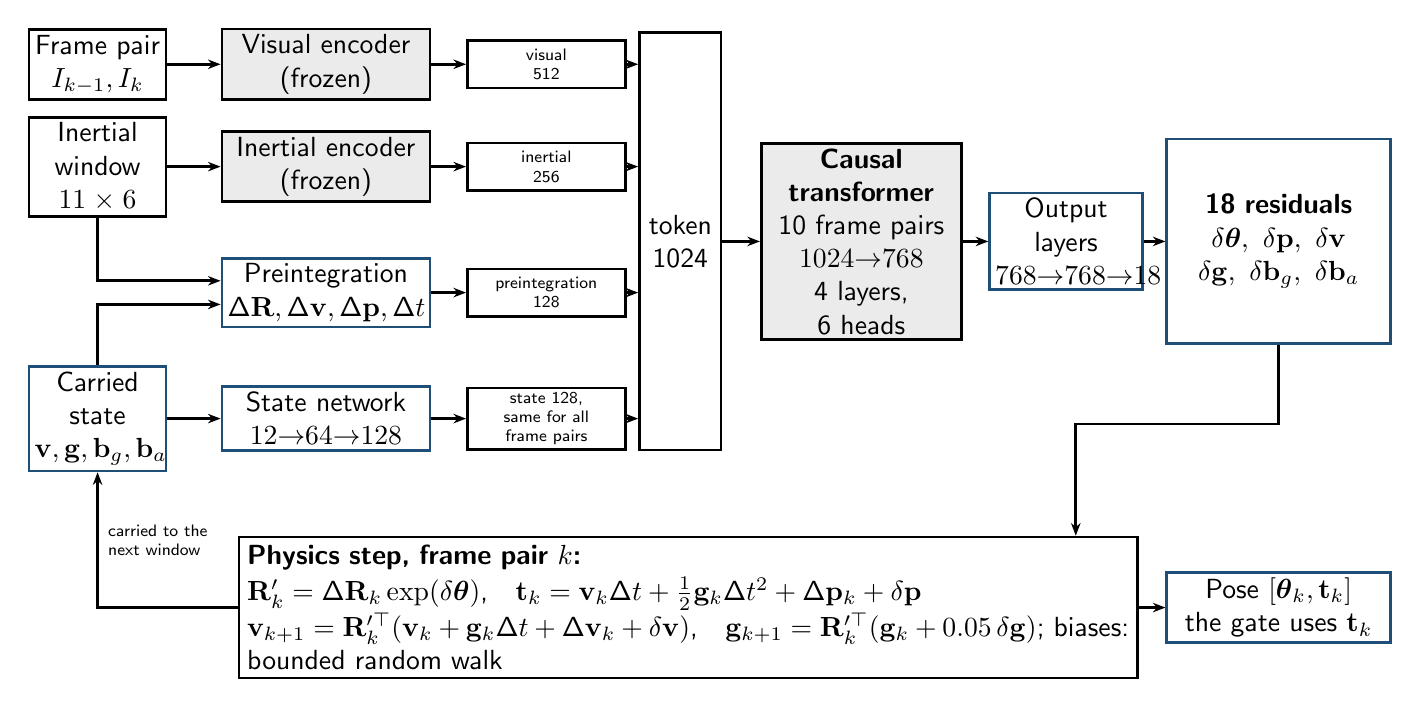
\begin{tikzpicture}[>={Stealth[length=1.6mm]}, every path/.style={line width=1pt},
  blk/.style={draw, align=center, inner sep=2pt, minimum height=8mm, text width=#1},
  blk/.default=22mm,
  inp/.style={blk=16mm},
  enc/.style={blk=#1, fill=black!8}, enc/.default=25mm,
  add/.style={blk=#1, draw=acc}, add/.default=25mm,
  tok/.style={draw, align=center, inner sep=1.5pt, font=\fontsize{6}{7}\selectfont, text width=19mm, minimum height=6mm}]
\node[inp] (img) at (0.9,0) {Frame pair\\$I_{k-1},I_k$};
\node[inp] (imu) at (0.9,-1.3) {Inertial window\\$11\times6$};
\node[blk=16mm, draw=acc] (st) at (0.9,-4.5) {Carried state\\$\mathbf v,\mathbf g,\mathbf b_g,\mathbf b_a$};
\node[enc] (venc) at (3.8,0) {Visual encoder\\(frozen)};
\node[enc] (ienc) at (3.8,-1.3) {Inertial encoder\\(frozen)};
\node[add] (pre) at (3.8,-2.9) {Preintegration\\$\DD\mathbf R,\DD\mathbf v,\DD\mathbf p,\DD t$};
\node[add] (smlp) at (3.8,-4.5) {State network\\$12{\to}64{\to}128$};
\node[tok] (tv) at (6.6,0) {visual\\512};
\node[tok] (ti) at (6.6,-1.3) {inertial\\256};
\node[tok] (tp) at (6.6,-2.9) {preintegration\\128};
\node[tok] (ts) at (6.6,-4.5) {state 128,\\same for all frame pairs};
\node[draw, align=center, minimum height=5.3cm, text width=8mm] (cat) at (8.3,-2.25) {token\\1024};
\node[blk=24mm, fill=black!8, minimum height=24mm] (tf) at (10.6,-2.25) {\textbf{Causal transformer}\\10 frame pairs\\$1024{\to}768$\\4 layers, 6 heads};
\node[add=18mm] (head) at (13.2,-2.25) {Output layers\\$768{\to}768{\to}18$};
\node[add=27mm, minimum height=26mm] (res) at (15.9,-2.25) {\textbf{18 residuals}\\$\delta\boldsymbol\theta,\ \delta\mathbf p,\ \delta\mathbf v$\\$\delta\mathbf g,\ \delta\mathbf b_g,\ \delta\mathbf b_a$};
\node[draw, inner sep=3pt, text width=112mm, align=left] (ph) at (8.4,-6.9) {\textbf{Physics step, frame pair $k$:}\\[1pt]
$\mathbf R'_k=\DD\mathbf R_k\exp(\delta\boldsymbol\theta)$,\quad $\mathbf t_k=\mathbf v_k\DD t+\tfrac12\mathbf g_k\DD t^2+\DD\mathbf p_k+\delta\mathbf p$\\[1pt]
$\mathbf v_{k+1}=\mathbf R_k'^{\top}(\mathbf v_k+\mathbf g_k\DD t+\DD\mathbf v_k+\delta\mathbf v)$,\quad $\mathbf g_{k+1}=\mathbf R_k'^{\top}(\mathbf g_k+0.05\,\delta\mathbf g)$;\ biases: bounded random walk};
\node[blk=27mm, draw=acc] (out) at (15.9,-6.9) {Pose $[\boldsymbol\theta_k,\mathbf t_k]$\\the gate uses $\mathbf t_k$};
\draw[->] (img) -- (venc); \draw[->] (imu) -- (ienc);
\draw[->] (imu.south) |- ([yshift=1.5mm]pre.west);
\draw[->] (st.north) |- ([yshift=-1.5mm]pre.west);
\draw[->] (st) -- (smlp);
\draw[->] (venc) -- (tv); \draw[->] (ienc) -- (ti); \draw[->] (pre) -- (tp); \draw[->] (smlp) -- (ts);
\foreach \t in {tv,ti,tp,ts} {\draw[->] (\t.east) -- (\t.east-|cat.west);}
\draw[->] (cat) -- (tf); \draw[->] (tf) -- (head); \draw[->] (head) -- (res);
\draw[->] (res.south) -- ++(0,-1.0) -| ([xshift=-8mm]ph.north east);
\draw[->] (ph.east) -- (out.west);
\draw[->] (ph.west) -| node[pos=0.75, right, font=\fontsize{6}{7}\selectfont, text width=17mm, align=left]{carried to the next window} (st.south);
\end{tikzpicture}}
\hoffset=-1in \voffset=-1in
\pdfpagewidth=\wd\figbox
\pdfpageheight=\ht\figbox \advance\pdfpageheight by \dp\figbox
\shipout\copy\figbox
\end{document}
